\section{Introduction}
\label{sec:intro}
In this lab, an amplifier with bandpass filter targeting a central frequency of 1kHz and gain of 40dB using an OP AMP was designed, simulated in ngspice and analysed using theoretical mathematical models.\\
 In the theoretical analysis section, the circuit's transfer funciton T(s) was used to calculate the expected output voltage for a wide range of frequencies, namely on the 1kHz central frequency. The input and output impedances were also calculated for the desired central frequency using circuit analysis methods. One must note that an ideal model of the OP AMP was used for these calculations. \\
 In the simulation section, the circuit was simulated using ngspice. The values for the central frequency obtained by the design, its input and output impedances and output voltage gain were obtained.\\
In the comparision section, values from both analysis are presented side by side and compared.\\ \\
The designed circuit is the following:

\begin{figure} [!htb] 
  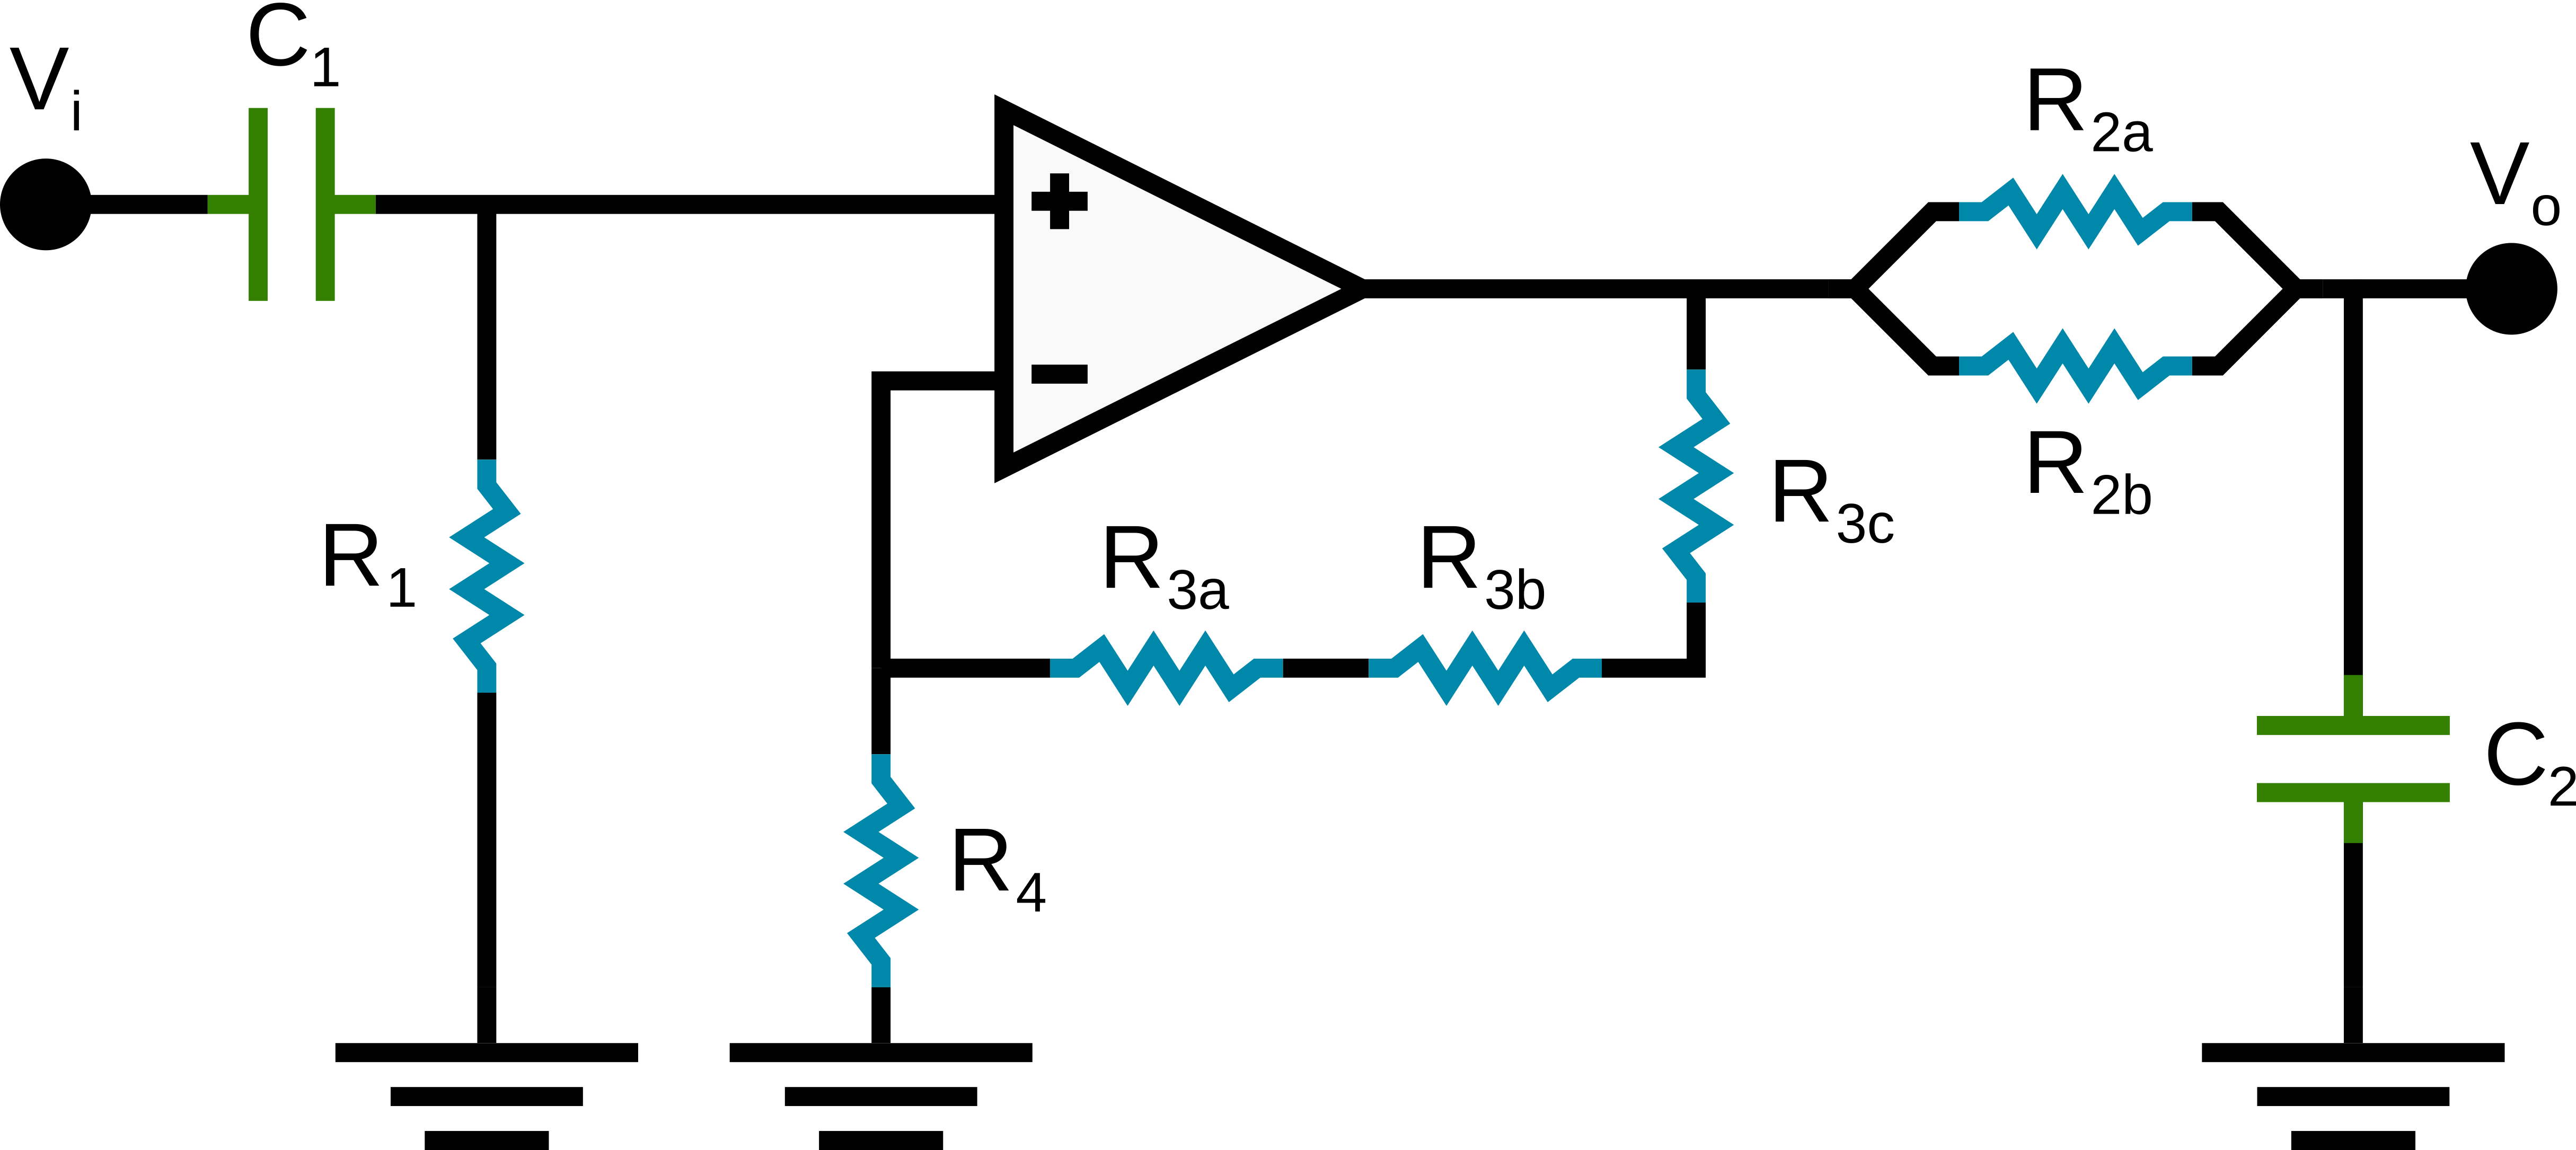
\includegraphics[width=\linewidth]{circuit.png}
  \vspace{1cm}
  \caption{Amplifier circuit}
  \label{fig:circuit}
  \hfill
\end{figure}

\begin{table}[h]
\centering
\begin{tabular}{|l|l|l|l|l|l|l|l|l|}
\hline
$R_{1}$    & $R_{2a}$   & $R_{2b}$   & $R_{3a}$     & $R_{3b}$     & $R_{3c}$     & $R_{4}$     & $C_{1}$ & $C_{2}$ \\ \hline
$1k\Omega$ & $1k\Omega$ & $1k\Omega$ & $100k\Omega$ & $100k\Omega$ & $100k\Omega$ & $10k\Omega$ & $220nF$ & $220nF$ \\ \hline
\end{tabular}
\caption{Components used}
\label{tab:my-table}
\end{table}


\FloatBarrier
